\documentclass[manuscript, letterpaper]{aastex6}
\bibliographystyle{aasjournal}

\usepackage{graphicx}
\usepackage[suffix=]{epstopdf}
\usepackage{natbib}
\usepackage{amsmath}
\usepackage{url}
\usepackage{xspace}


% from here: https://github.com/dfm/peerless/blob/master/document/ms.tex#L19-L69
% ----------------------------------- %
% start of AASTeX mods by DWH and DFM %
% ----------------------------------- %
\setlength{\voffset}{0in}
\setlength{\hoffset}{0in}
\setlength{\textwidth}{6in}
\setlength{\textheight}{9in}
\setlength{\headheight}{0ex}
\setlength{\footnotesep}{0in}
\setlength{\topmargin}{-\headsep}
\setlength{\oddsidemargin}{0.25in}
\setlength{\evensidemargin}{0.25in}
\linespread{0.54} % close to 10/13 spacing in ``manuscript''
\setlength{\parindent}{0.54\baselineskip}
%\hypersetup{colorlinks = false}
\makeatletter % you know you are living your life wrong when you need to do this
\long\def\frontmatter@title@above{
\vspace*{-\headsep}\vspace*{\headheight}
\noindent\footnotesize
{\noindent\footnotesize\textsc{\@journalinfo}}\par
{\noindent\scriptsize Preprint typeset using \LaTeX\ style AASTeX6\\
With modifications by David W. Hogg, Daniel Foreman-Mackey, Boris Leistedt
}\par\vspace*{-\baselineskip}\vspace*{0.625in}
}%
\makeatother
% Section spacing:
\makeatletter
\let\origsection\section
\renewcommand\section{\@ifstar{\starsection}{\nostarsection}}
\newcommand\nostarsection[1]{\sectionprelude\origsection{#1}}
\newcommand\starsection[1]{\sectionprelude\origsection*{#1}}
\newcommand\sectionprelude{\vspace{1em}}
\let\origsubsection\subsection
\renewcommand\subsection{\@ifstar{\starsubsection}{\nostarsubsection}}
\newcommand\nostarsubsection[1]{\subsectionprelude\origsubsection{#1}}
\newcommand\starsubsection[1]{\subsectionprelude\origsubsection*{#1}}
\newcommand\subsectionprelude{\vspace{1em}}
\makeatother
\widowpenalty=10000
\clubpenalty=10000
\sloppy\sloppypar
% ------------------ %
% end of AASTeX mods %
% ------------------ %

\journalinfo{Prepared for ApJ}



\newcommand{\ie}{{\textit{i.e.}~}}
\newcommand{\eg}{{\textit{e.g.},~}}
\newcommand{\equref}[1]{{\xspace}Eq.~(\ref{#1})}
\newcommand{\figref}[1]{{\xspace}Fig.~\ref{#1}}
\newcommand{\figrefs}[2]{{\xspace}Figs.~\ref{#1}~and ~\ref{#2}}
\newcommand{\equrefbegin}[1]{{\xspace}Equation~(\ref{#1})}
\newcommand{\figrefbegin}[1]{{\xspace}Figure~\ref{#1}}
\newcommand{\secref}[1]{{\xspace}Sec.~\ref{#1}}
\renewcommand{\d}{{\mathrm{d}}}
\newcommand{\equ}[1]{\begin{equation}#1\end{equation}}
\newcommand{\eqn}[1]{\begin{eqnarray}#1\end{eqnarray}}
\renewcommand{\vec}[1]{\bmath{#1}}
\newcommand{\negsp}[1]{\hspace*{-#1mm}}

\newcommand{\gal}{g}
\newcommand{\nobj}{{N_{\rm stars}}}
\newcommand{\band}{b}

\newcommand{\todo}[1]{\textcolor{blue}{[TODO: #1]}}
\newcommand{\bl}[1]{\textcolor{blue}{[BL: #1]}}
\newcommand{\dwh}[1]{\textcolor{cyan}{[DWH: #1]}}


\begin{document}

 
\title{Shrinking stellar distance uncertainties\\
 with color-magnitude information \\
  but no use of physical stellar models}
  
\shorttitle{Shrinking distance errors with color--magnitude information}
\shortauthors{Leistedt et al}


\author{
	Boris~Leistedt\altaffilmark{1,2},
	David~W.~Hogg\altaffilmark{1,3,4}
	\textit{Add your name here}
	}


  \altaffiltext{1}{Center for Cosmology and Particle Physics, Department of Physics, \\ New York University, 726 Broadway, New York, NY 10003, USA}
  \altaffiltext{2}{NASA Einstein Fellow}
  \altaffiltext{3}{Center for Data Science, New York University, 60 Fifth Avenue, New York, NY 10011, USA}
  \altaffiltext{4}{Flatiron Institute, 162 Fifth Avenue, New York, NY 10010, USA}
  

\begin{abstract}
We present a hierarchical probabilistic model for improving parallax-based stellar distances estimates using color--magnitude information. 
This is achieved with a data driven model of the color--magnitude diagram, not relying on stellar models but instead on the  relative abundances of stars in color--magnitude cells, which are inferred from noisy magnitudes and parallaxes using an efficient sampling method.
This approach is equivalent to deconvolving observational errors into a probabilistic, noiseless color--magnitude diagram, which can be useful for a range of applications. 
We focus on leveraging color--magnitude information to provide more accurate stellar distance estimates.
We demonstrate the power of this approach on 1.4 million stars in the Gaia TGAS sample which have APASS magnitudes.
We find that distance estimates are significantly improved for the noisiest parallaxes and densest regions of the color--magnitude diagram. 
In particular, the average distance signal-to-noise and uncertainty improve by 26\% and 40\%, respectively, with 12\% of the objects having the latter reduced by a factor of 2.
We make our improved distance estimates publicly available.
\end{abstract}

\keywords{Stellar distances, probabilistic hierarchical models.} 

\newpage
%%%%%%%%%%%%%%%%%%%%%%%%%%%%%%%%%%%%%%
\section{Introduction}

Parallaxes are ubiquitous for determining stellar distances.
However, they are grow noisier for faint, distance stars, which populate most of the Galaxy. 
In particular, the resulting distance errors, under a Gaussian approximation, are proportional to the parallax error divided by the parallax squared.
This makes difficult to determine the distances above a few kilo parsecs (kpc). 
The typical noise of the Gaia DR1 data is

Luckily, stellar distances can also be determined from spectral information.
In particular, it is well known that the vast majority of stars live in compact regions of the color--magnitude space.
Thus, photometric information (\ie apparent magnitudes) can complement parallax information and prove crucial to determine distances.
However, theoretical models predict narrow tracks in color--magnitude (\ie tracks), and fail to account for the diversity of real objects.
Using those as priors for inferring the distances may bias the estimates.
In this paper, we present a purely data-driven approach for constructing a color--magnitude diagram and account for this diversity. 

Our approach relies a standard property of hierarchical probabilistic models: a large number of noisy observations (here, noisy parallaxes and magnitudes) can be used to construct an estimate of the underlying distribution (a color--magnitude diagram), which in turn shrinks the uncertainties on their individual properties (the distances).
In other words, \textit{the whole is greater than the sum of the parts}: stellar distance estimates can be improved by simultaneously analysing all the available data.
This is particularly relevant for Gaia which will soon provide hundreds of millions of sources with parallax, proper motion, and multicolor information.
This is an opportunity to construct accurate models of the distribution of magnitudes, colors, dust, and stellar densities in the Galaxy, without external data. 
Those models will in turn significantly improve our estimates of the intrinsic properties of individual stars.
The core goal of this paper is to demonstrate how one aspect of this hierarchical inference can be done in practice. 
We focus on evaluating the shrinkage of distance estimates obtained by constructing a flexible color--magnitude diagram based on the joint analysis of millions of noisy parallaxes and apparent magnitudes.

We make a number of simplifying assumptions to make our demonstration more transparent, such as adopting uninformative distance priors and point estimates of dust corrections. 
Those assumptions could be relaxed by inferring the 3D distribution of stars and dust jointly with the color--magnitude diagram.
In fact, they ultimately \emph{should} be relaxed in order to properly infer the full multivariate distribution of stellar colors and distances in the presence of non-trivial structure on the three-dimensional stellar density and dust in our Galaxy.

This paper is structured as follows: our model and inference framework are described in \secref{sec:model}, and applied to the Gaia data in \secref{sec:application}. 
Conclusions and perspectives are presented in \secref{sec:concl}.

%%%%%%%%%%%%%%%%%%%%%%%%%%%%%%%%%%%%%%
\section{Model}\label{sec:model}


\begin{table} %%%%
\centering
\begin{tabular}{cl}
\hline
$s$	&	object index (the $s$-th star)\\
$d_s, \varpi_s, M_s, C_s$	&	true distance, parallax, absolute magnitude, and color	\\
$\hat{\varpi}_s, \sigma_{\hat{\varpi}_s}^2$ 	&	parallax estimate and its variance\\
$\hat{m}_s, \hat{C}_s, \sigma^2_{\hat{m}_s}, \sigma^2_{\hat{C}_s}$ 	&	apparent magnitude and color estimates, and their variances\\
$b_s$	&	index of the color--magnitude bin of the $s$th object\\
\hline
$b$	&	generic index of color--magnitude bin\\
$n_b$	& 	object count in the $b$-th color--magnitude bin  \\
$\{n_b\}$	&	set of all galaxy counts $n_b$, summing to $\nobj$\\
$f_b$	&	fractional galaxy count in the $b$-th color--magnitude bin  \\
$\{f_b\}$	&	set of all fractional bin counts $f_b$, summing to $1$\\
$\{ d_s, b_s\}$	&	distances and bins of all stars in the sample	\\
$\{ \hat{m}_s, \hat{C}_s \}$ &	all magnitude and color estimates\\
\hline
\end{tabular}
\caption{Summary of our notation. }
\label{tab:notation}
\end{table} 

We consider a set of stars indexed as $s=1, \cdots, \nobj$, each characterized by a distance $d_s$, an absolute magnitude $M_s$, and a color $C_s$. 
The magnitude and color are taken with respect to an arbitrary reference band.
We only consider one color for simplicity, but it should be noted that the model and method presented below can be straightforwardly extended to multiple magnitudes and colors.

Intrinsic properties like distance and absolute magnitude are not directly observable.
Instead, what we have at our disposal is a set of apparent magnitude and parallax measurements.  
The estimate of the parallax is denoted $\hat{\varpi}_s$ and is assumed to have a Gaussian variance $\sigma_{\hat{\varpi}_s}^2$.
We will consider two magnitudes only, $\hat{m}_s$ and $\hat{m}^\prime_s$, assumed to be uncorrelated and have Gaussian variances $\sigma_{\hat{m}_s}^2$ and $\sigma_{\hat{m}^\prime_s}^2$.
We will use the first one $\hat{m}_s$ as a reference magnitude for inferring the absolute magnitude $M_s$, and the second one to form a color estimate $\hat{C}_s =\hat{m}^\prime_s - \hat{m}_s $ with Gaussian variance $\sigma_{\hat{C}_s}^2 = \sigma_{\hat{m}_s}^2 + \sigma_{\hat{m}^\prime_s}^2$.

We aim at estimating the distance $d_s$ of each star from the noisy data $\hat{m}_s$,  $\hat{C}_s$ and $\hat{\varpi}_s$. 
While distance is directly connected to the parallax via $\varpi_s=1/d_s$, it is also informed by the apparent magnitude since $m_s = M_s + 5\log_{10} d_s$ where $d_s$ is expressed in units of $10$ pc.
Note that when only the apparent magnitude is available, distance and absolute magnitude are degenerate and cannot be disentangled. 
This degeneracy is partially broken with the parallax information.
Here, we seek to incorporate the knowledge that stars do not have arbitrary colors and magnitude.
The way this information enters distance estimates is made obvious by writing the posterior probability distribution on the distance,
\eqn{
	p(d_s | \hat{m}_s, \hat{C}_s, \hat{\varpi}_s) = \int \d M_s \ \d C_s \ p\bigl(\hat{m}_s, \hat{C}_s, \hat{\varpi}_s \bigr\rvert M_s, d_s, C_s\bigr) \ p\bigl( M_s, d_s, C_s \bigr) \label{eq:naivedistposterior}.
}
This integral marginalizes over the true absolute magnitude and color.
This might be expensive to perform numerically, but the choices we will make below will allow us to execute it analytically.

The first term of \equref{eq:naivedistposterior} is a likelihood function, and the second term is the prior. 
Assuming that the magnitude and parallax estimates are independent, the likelihood function factorizes as the product of two terms, 
\equ{
	p\left(\hat{\varpi}_s \bigr\rvert d_s\right) = \mathcal{N}\bigl(\hat{\varpi}_s - d_s^{-1};\sigma_{\hat{\varpi}_s}^2 \bigr),\label{eq:parallaxlike}
}
and
\equ{
	p\bigl(\hat{m}_s, \hat{C}_s \bigr\rvert M_s, d_s, C_s\bigr)  =  \mathcal{N}\bigl( M_s + 5\log_{10}d_s  -\hat{m}_s ;\sigma_{\hat{m}_s}^2 \bigr) \  \mathcal{N}\bigl(\hat{C}_s - C_s;\sigma_{\hat{C}_s}^2 \bigr),
}
where we have neglected the correlation between the observed magnitudes (and thus color and magnitude). 
This could easily be added.

The final term, $ p\bigl( M_s, d_s, C_s \bigr) $, is the prior knowledge about the distances, magnitudes, and colors of stars. 
\todo{Cite literature and discuss how this is usually handled.}

We will adopt a uniform distance prior and focus on the magnitude--color term, which we parametrize as $p\left(M_s, C_s  \bigr\rvert \{ f_{b} \} \right) $.
We construct a model of the relative abundance of objects in color--magnitude cells (\ie in two dimensions: absolute magnitude and color).
The color--magnitude distribution is described as a linear mixture of $B$ components,
\equ{
	p\left(M_s, C_s  \bigr\rvert \{ f_{b} \} \right) = \sum_{b=1}^B f_b \ K_b(M_s, C_s),
} 
with $K_b$ the kernel of the $b$th component. 
In other words, the parameters $\{ f_{b} \}$ refer to the relative probabilities of finding objects in the various cells, and must sum to one ($\sum_b f_b = 1$).

For the kernels, we adopt Gaussian distributions to make the integral of \equref{eq:naivedistposterior} analytically tractable.
The $b$-th kernel will be centered at $(\mu_{b,0}, \mu_{b,1})$ and have a diagonal covariance $(\sigma_{b,0}^2, \sigma_{b,1}^2)$.
We take $\mu_{b+1,0}-\mu_{b,0} = \sigma_{b,0}$ and $\sigma_{b,0}$ constant (similarly for the color dimension) to uniformly and contiguously tile a rectangular region of interest in color--magnitude space. 
With this parameterization, the integral of \equref{eq:naivedistposterior} is tractable and leads to
\eqn{
	p(d_s | \hat{m}_s, \hat{C}_s, \hat{\varpi}_s, \{ f_{b} \})  \ &\propto&  \ \sum_b\ f_b \ \mathcal{N}\bigl(\hat{\varpi}_s - d_s^{-1};\sigma_{\hat{\varpi}_s}^2 \bigr) \\ 
	&& \quad\quad \times \ \ \mathcal{N}\bigl( \mu_{b_s,0} + 5\log_{10}d_s  -\hat{m}_s ;\sigma_{\hat{m}_s}^2 + \sigma_{b_s,0}^2 \bigr) \nonumber\\ 
	&& \quad\quad \times \ \ \mathcal{N}\bigl(\hat{C}_s - \mu_{b_s,1};\sigma_{\hat{C}_s}^2 + \sigma_{b_s,1}^2 \bigr). \label{eq:distposterior}\nonumber
}

Finally, to facilitate parameter inference, we will introduce a latent variable $b_s$ denoting the bin the $s$th object belongs to.
Then, we can equivalently write the color--magnitude model as
\eqn{
	p\left(b_s \bigr\rvert \bigl\{ f_b \bigr\}\right) \ &=& \ f_{b_s} \\ 
	p\left(M_s, C_s \bigr\rvert b_s \right) \ &=& \ \mathcal{N}\bigl(M_s - \mu_{b,0};\sigma_{b,0}^2 \bigr)  \ \mathcal{N}\bigl(C_s - \mu_{b,1};\sigma_{b,1}^2 \bigr).\nonumber
}
Our notation is summarized in Table~\ref{tab:notation}.

Note that in all of the above we have assumed that all magnitudes are properly dereddenned, \ie that the absorption by interstellar dust has been corrected for.
As discussed below, we will use the distance point estimate $1/\hat{\varpi}_s$ for performing this correction.
While this is formally incorrect (since the reddenning correction depends on distance which is a parameter we are inferring), this approximation will be sufficient for the demonstration below.


%%%%%%%%%%%%%%%%%%%%%%%%%%%%%%%%%%%%%%
\subsection{Inference}

Assuming that the kernel locations $\{  (\mu_{b,0}, \mu_{b,1}) \}$ and covariances $\{(\sigma_{b,0}^2, \sigma_{b,1}^2)\}$ are fixed, our color--magnitude model is fully described by the relative amplitudes $\{ f_{b} \}$. 
If they are fixed by prior knowledge (\eg external data or stellar models), then one can use \equref{eq:distposterior} to infer the distance of each object using both parallax and color--magnitude information.
Here, we seek to infer $\{ f_{b} \}$ too.
Thus, the full posterior of interest is $p(\{ d_s \}, \{ f_{b} \} | \{ \hat{m}_s, \hat{C}_s, \hat{\varpi}_s \})$, which has $B + \nobj$ parameters.

Given the number of parameters and the natural degeneracies between magnitudes and distances, standard sampling techniques may be difficult to apply.
However, the inference is greatly simplified by focusing on $p(\{ b_s \}, \{ f_{b} \} | \{ \hat{m}_s, \hat{C}_s, \hat{\varpi}_s \})$, where distances are marginalized over.
We adopt a Gibbs sampling strategy, which consists of alternating draws from the conditional distributions of $\{ b_s \}$ and $\{ f_{b} \}$.
At the $i$th iteration, we will draw new values of the $\{ f_{b} \}$ and $\{b_s\}$ parameters given the values of the previous iteration.
In other words, we first draw $\{ f_{b} \}^{(i)}$ given $\{b_s\}^{(i-1)}$ (and the data), and for each object then draw $b_s^{(i)}$ given $\{ f_{b} \}^{(i)}$ (and the data). 
The sequence $\{ f_{b} \}^{(i)},\{b_s\}^{(i)}$ for $i=1, \cdots, N_\mathrm{samples}$ forms a Markov Chain with the target posterior distribution of interest as equilibrium distribution.
This allows us to avoid the magnitude--distance degeneracies and exploit other properties of our model, such as conjugate priors.
We now detail how to draw from the correct conditional distributions.

The first draw is fairly standard: with the bin locations $\{b_s\}$ fixed, the fractional weights $\{ f_{b} \}$ follow a Dirichlet-multinomial distribution (also known as Dirichlet compound multinomial distribution) entirely determined by $\{n_b \}$, with $n_b$ the number of objects in the $b$-th bin.
All the other parameters enter the constant proportionality factor, so the target conditional distribution is
\eqn{
	p\left(\bigl\{ f_b \bigr\} \bigr\rvert \bigl\{ d_s, b_s, \hat{m}_s, \hat{C}_s, \hat{\varpi}_s \bigr\} \right) \ = \ p\bigl( \bigl\{ f_b \bigr\} \bigr\rvert \{n_b \} \bigr) \ \propto\  \prod_b \frac{ f_b^{n_b} }{n_b !},
}
where we have assumed the simplest uninformative prior for the relative amplitudes, \ie that they are positive and normalized to one, \ie $p(\bigl\{ f_b \bigr\}) = \delta^D(1 - \sum_b f_b) \prod_b \Theta(f_b)$, where $\delta^D$ is the Dirac delta function and $\Theta$ the step function.
Given the number counts $\{n_b \}$, one can draw $\{ f_b \}$ from this distribution using standard tools for Dirichlet draws, or manually draw $\gamma_b \sim \mathrm{Gamma}(n_b + 1)$ and take $f_b = \gamma_b / \sum_b' \gamma_b'$.

The next and final step of the Gibbs sampler is to draw the bins $\{b_s\}$ given the amplitudes $\{f_b\}$. 
Even though this can be performed independently (thus, in parallel) over objects, this may not look simple since we have to marginalize over the distances, and the target conditional distribution to sample is
\eqn{
	p\left(b_s \bigr\rvert \bigl\{ f_b \bigr\}, \hat{m}_s, \hat{C}_s, \hat{\varpi}_s\right) \ &\propto& \  \int p\left(b_s, d_s \bigr\rvert \bigl\{ f_b \bigr\}, \hat{m}_s, \hat{C}_s, \hat{\varpi}_s\right)  \mathrm{d} d_s.
}  
However, closer examination reveals that the bins can be simply drawn from a multinomial distribution with amplitudes given by
\eqn{
	p\left(b_s \bigr\rvert \bigl\{ f_b \bigr\}, \hat{m}_s, \hat{C}_s, \hat{\varpi}_s\right) \ &\propto& \ f_{b_s}  g_{b_s}
} 
with
\equ{
	g_{b_s} = \int \mathcal{N}\bigl( \mu_{b_s,0} + 5\log_{10}d_s  -\hat{m}_s ;\sigma_{\hat{m}_s}^2 + \sigma_{b_s,0}^2 \bigr)   \mathcal{N}\bigl(\hat{C}_s - \mu_{b_s,1};\sigma_{\hat{C}_s}^2 + \sigma_{b_s,1}^2 \bigr) p(d_s)  \mathrm{d}  d_s.
}
Since we keep the kernel locations and covariances fixed, those weights can be precalculated via $\nobj$ independent one-dimensional integrals.
We evaluate them numerically given that the integrand is simple and the integration can be tuned easily. 
If this operation were prohibitive, or if the kernel parameters were not kept fixed, one could sample the distance $d_s$ (jointly of conditionally on the bin $b_s$).
Since the kernels and the likelihood admit simple gradients and Hessians, one could use Hamiltonian Monte Carlo REF to efficiently sample those parameters simultaneously for all objects.


%%%%%%%%%%%%%%%%%%%%%%%%%%%%%%%%%%%%%%
\subsection{Discussion}

\begin{figure}
\hspace*{-3mm}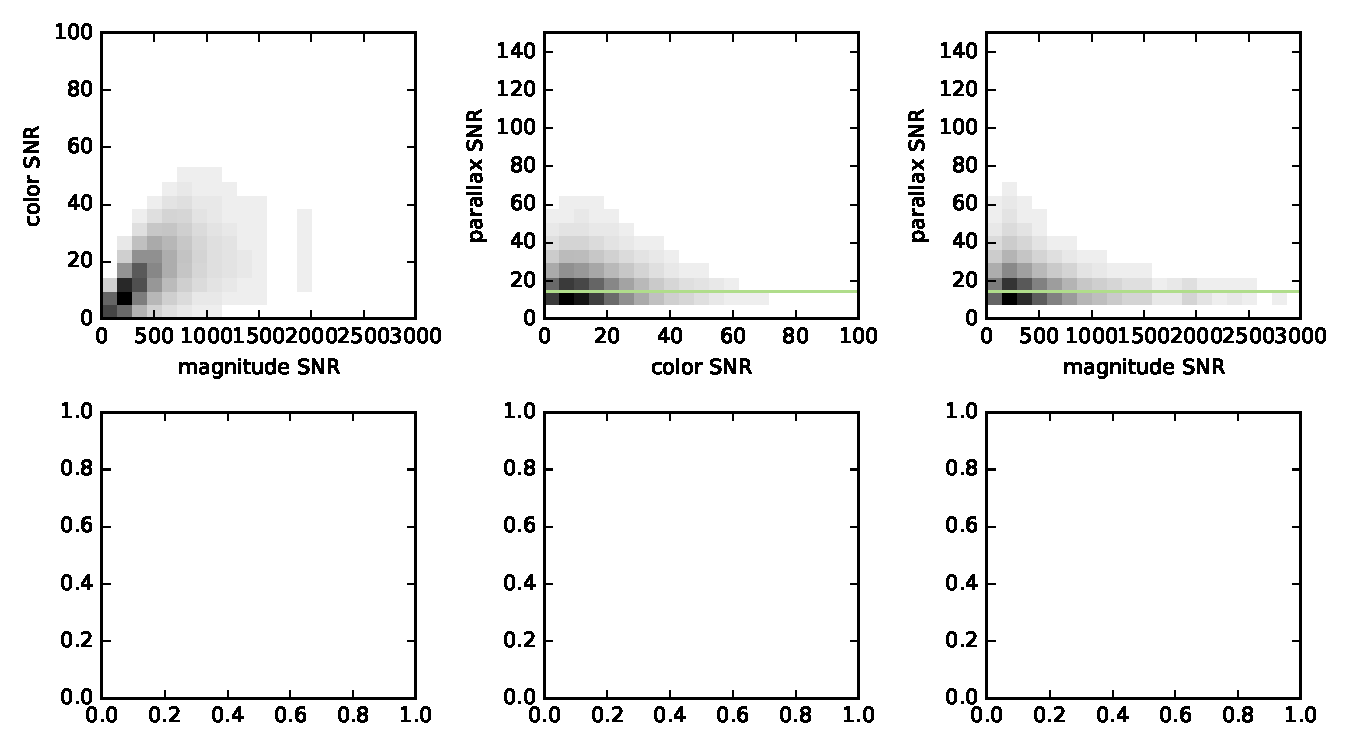
\includegraphics[width=15.75cm]{datasummary.pdf}
\caption{Distributions of the magnitude, color, and parallax signal-to-noise ratios (SNR) of the Gaia TGAS+APASS data we train and validate our model on. The line indicates the parallax SNR level used to split the data into two sub-samples containing the `best' and `worst' parallaxes. The right panel shows the average parallax SNR in color--magnitude cells, illustrating how the upper part of the color--magnitude diagram is dominated by low-SNR objects. Reconstructing the noiseless color--diagram requires an inference framework capable of correctly dealing with uncertainties in colors, magnitudes, and parallaxes.}
\label{fig:datasummary}
\end{figure}

We now briefly discuss the advantages and limitations of our approach.

First, we restricted our attention to the color--magnitude diagram, and neglected any dependency on other quantities such as galactic latitude.
In particular, we adopted uniform distance priors.
This can be corrected by adopting or constraining models of the 3D distribution stellar densities, described by kernel mixtures, for example. 
Although this extension is technically trivial, we have not developed it since we focus on how color--magnitude information informs distance estimates.
Similarly, our framework could be extended to other observables such as proper motions and velocities.

Second, our kernel mixture model offers a significant amount of freedom for describing the color--magnitude diagram.
Changing the kernels does not affect our inference framework, unless they are not differentiable, in which case it is not possible to use Hamiltonian Monte Carlo.
Analytic marginalization of true magnitudes and colors are made possible by adopting Gaussian kernels. 
Furthermore, we have not optimized the positions and sizes of the kernels, unlike in standard Gaussian Mixture models. 
Compared to those, our tiling of color--magnitude space requires more components (many of which are zero) but is easy to initialize, and also converges quickly. 

Third, we have assumed that the magnitudes are dust-corrected. 
However, dust extinction depends on distance, which is a parameter of our model, inferred from parallax and color--magnitude information.
Furthermore, reliable 3D dust maps are only available and reliable for a limited region of space.
Thus, in principle, dust corrections should really be inferred jointly with the absolute magnitudes and colors of the data at hand. 
The approximation we use here is sufficient for inferring the color--magnitude diagram and demonstrating the improvement of distance estimates.

%%%%%%%%%%%%%%%%%%%%%%%%%%%%%%%%%%%%%%
\section{Application to Gaia TGAS}\label{sec:application}

\begin{figure}
\hspace*{-3mm}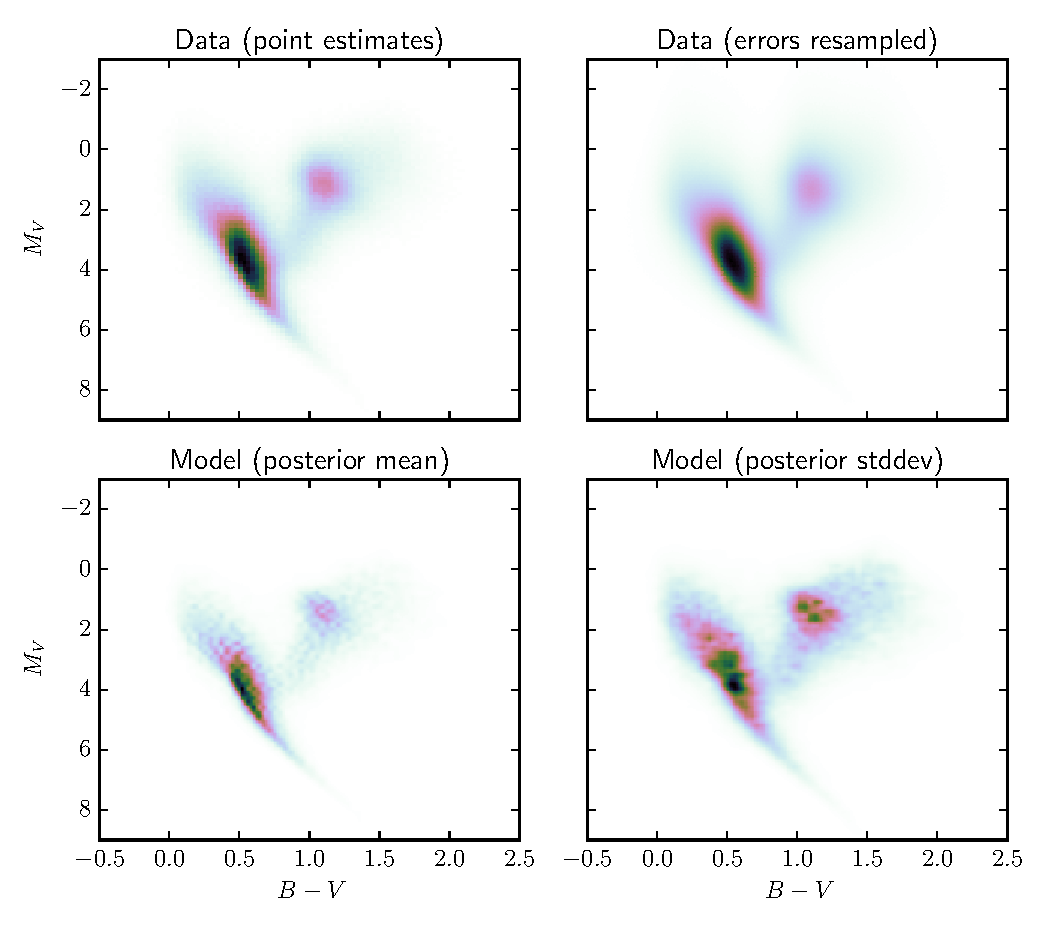
\includegraphics[width=15cm]{colmagdiag_mainsample.pdf}
\caption{Upper panels: color--diagram based on the noisy data, obtained with magnitude and parallax point estimates (left) and by sampling parallaxes, magnitude and color based on the measurements and their errors (right). Middle and right: mean and standard deviation of our model, which is the result of deconvolving all observational errors of the data shown in the upper panels and in \figref{fig:datasummary} into a noiseless color--magnitude diagram described as a mixture of Gaussians tiling the color--magnitude region of interest. }
\label{fig:colmagdiag_mainsample}
\end{figure}


\begin{figure}
\hspace*{-3mm}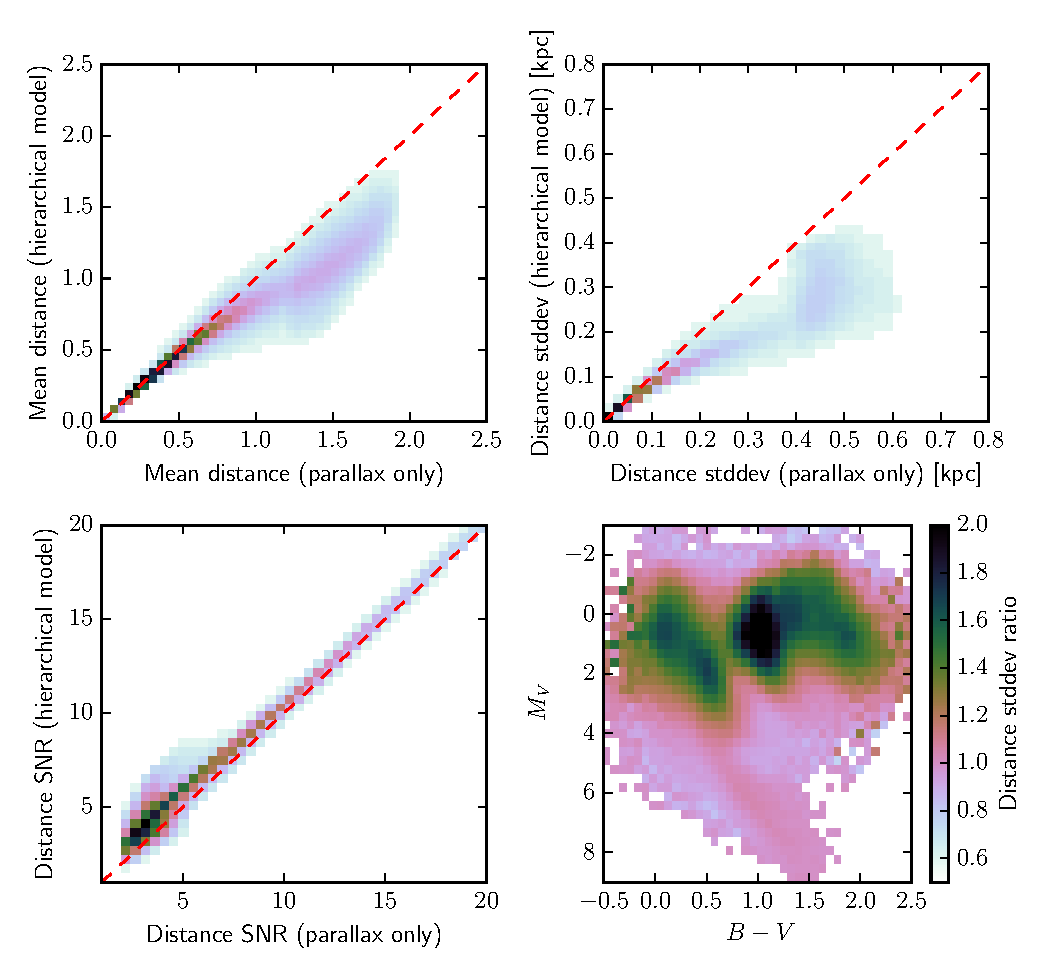
\includegraphics[width=15.5cm]{colmagdiag_mainsample_dist.pdf}
\caption{Distances obtained when sampling the hierarchical model which produced the color--diagram shown in \figref{fig:colmagdiag_mainsample}. 
The first three panels shows the change in the mean, standard deviation, and SNR of the distance estimate (based on the posterior distribution), with the number counts in logarithmic scale. The final panel shows the ratio of standard deviations placed in the color--diagram (standard method over hierarchical model). The shrinkage of the uncertainties is a consequence of the hierarchical natural of the model, and is most efficient for low-SNR objects and the densest parts of the color diagram.}
\label{fig:colmagdiag_mainsample_dist}
\end{figure}


\begin{figure}
\hspace*{-2mm}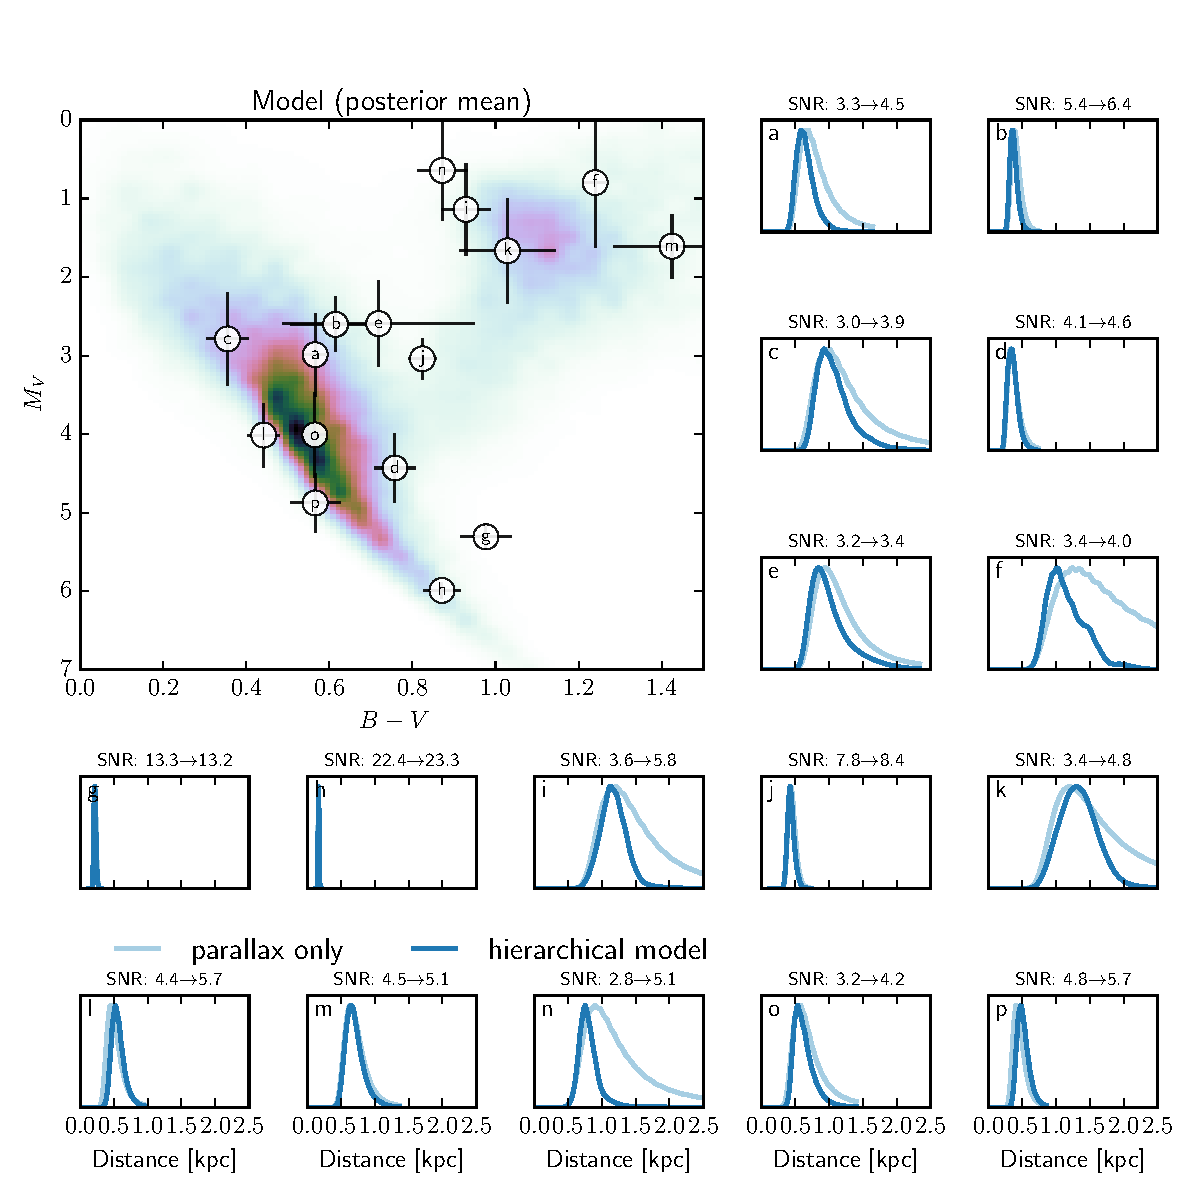
\includegraphics[width=15.7cm]{model_dist_pdfs.pdf}
\caption{Posterior distributions on the distances of a few objects involved in constraining the model shown in \figrefs{fig:colmagdiag_mainsample}{fig:colmagdiag_mainsample_dist}. 
The improvement in distance SNR is also shown. The objects are also placed on the inferred color--magnitude diagram, to highlight that the shrinkage is most efficient for low-SNR objects and the densest parts of the color diagram.}\label{fig:model_dist_pdfs}
\end{figure}

We consider the Gaia data \citep{gaia}, specifically the first data release (DR1) of the Tycho-Gaia astrometric solution\citep[hereafter TGAS][]{gaia_dr1}.
We restrict our attention to the objects with valid B and V magnitudes from the AAVSO Photometric All Sky Survey (APASS) Data Release 9 \citep{munari2014, hendenmunari2014}. 
We also remove objects with parallax signal-to-noise ratio (SNR) lower than 1. 
This leads to 1.4 million objects with magnitude, color, and parallax information. 
We don't apply more stringent parallax or color cuts since the purpose of our method is exactly to construct a color--magnitude model from both low and high-SNR objects. 
Finally, we apply dust corrections based on position and distance point estimate ($1/\hat{\varpi}$) with the three-dimensional dust map of \cite{Green2015bayestar}. 
For large distances when the latter is undefined we use corrections from the 2D dust map of \cite{sfd1998}.
Our data sample is summarized in \figref{fig:datasummary}, which shows the magnitude, color, and parallax SNR distributions.
The bulk of the objects has parallax SNR lower than 10 and is at $M_V  < 4$, in the upper part of the color--magnitude diagram.
This highlights the need for a correct inference framework that exploits all objects, since focusing on high-SNR objects would bias the results and prevent us from correctly inferring the fainter regions of the color--magnitude space.

We create a validation sample by randomly extracting 10\% of the objects. 
As detailed below, we will add significant amount of noise to the parallax estimates and verify that our framework improves the distances consistently with the original values. 
We also split the main sample according to parallax SNR, into two samples of equal size containing the `best' and a `worst' parallaxes. 
We perform the inference on those two samples as well as the combined one. 
For each of the three samples, we use the Gibbs sampler presented above to draw 10,000 samples of the fractional bin weights, bins, and distances. 

The mean and standard deviation of the resulting color--magnitude diagram (with bins and distances marginalized) are presented in \figref{fig:colmagdiag_mainsample}.
The top panels also show the input data, with and without resampling according to the estimates and their errors.
As expected, the recovered models are significantly narrower than the data since we are effectively deconvolving observational errors to produce a noiseless color--magnitude diagram. 
Most classical features are recovered: the main sequence, its turn-over, and the giant branch.

\figref{fig:colmagdiag_mainsample_dist} shows the stellar distances with bins and color--magnitude model marginalized over. 
We compute the mean and standard deviation using samples of the joint posterior distribution. 
We also compute mean and standard deviation using samples of the parallax likelihood, \ie not using our hierarchical model but only the parallax information of \equref{eq:parallaxlike}.
Note that the posterior distributions are not Gaussian, as expected and also shown below. 
Nevertheless, the standard deviation provides a useful metric. 
We measure that on average the distance SNR improves by 26\% and the distance uncertainty decreases by 40\%.
We find that 12\% of the objects have their distance uncertainty halved after the inclusion of color--magnitude information via our hierarchical model.
This shrinkage of the distance uncertainties is most efficient in the most densely populated regions of color--magnitude space.
\figref{fig:model_dist_pdfs} shows the distance posterior distributions obtained with our method for a few randomly chosen object, further illustrating the shrinkage of the uncertainties.
For clarity we have smoothed the distance samples obtained with the Gibbs sampler.
We also place these objects in the color--magnitude diagram.
The errors are obtained by resampling.

\figref{fig:colmagdiag_othersamples} shows the  mean and standard deviation of the color--magnitude diagram resulting from performing the inference on the subsamples with parallax SNR cuts (\ie splitting our main sample at parallax SNR of 8). 
Those demonstrate that including the noisiest objects is essential for correctly inferring the fainter regions of magnitude space.
The main sequence is well recovered with the high-SNR objects, while the red giant branch is barely detected. 
By contrast, it is well recovered with the low-SNR objects, but the main sequence is then partially erased.
This is a natural consequence of the SNR increasing with absolute magnitude.
This highlights the importance of a correct probabilistic framework, capable of correctly exploiting data with heterogeneous noise to reconstruct the noiseless color--magnitude diagram.

We now turn to the validation sample. 
Since we do not know the true distances for those objects, we take a different approach: we add noise to the parallax estimate, at a level equal to ten times the parallax error. 
We then compute the posterior distribution on the distance (on a distance grid) using the parallax likelihood as well as the distance posterior. We simply use the mean model shown in \figref{fig:colmagdiag_mainsample} as a color-magnitude prior. 
The results are shown in \figref{fig:cv_metrics}.
Given that those objects have significant amounts of noise, causing the distance posterior distribution to be highly non-Gaussian, the mean distance overestimates the true distance (the original parallax-based estimate). 
The hierarchical model significantly decreases this effect, \ie improves the distance estimates both in terms of mean and uncertainty, demonstrating the validity of our inference scheme.

Finally, we perform an additional test of our method on open clusters.
We retrieve the coordinates, distances, and proper motions, of known open clusters from the WEBDA database\footnote{www.univie.ac.at/webda/}.
From our TGAS-APASS sample, we select cluster member candidates for each cluster in a radius corresponding to 3 pc.
\figref{fig:cv_metrics} shows the result of applying our framework to those objects for a few selected clusters, \ie using the color--diagram inferred above to inform the distance posterior distribution.
The distances SNRs are improved and the point estimates change towards the open cluster distance, even though the improvement is relatively modest due to the proximity of those clusters and the good parallax SNR of the cluster members we identified.

\begin{figure}
\hspace*{-4mm}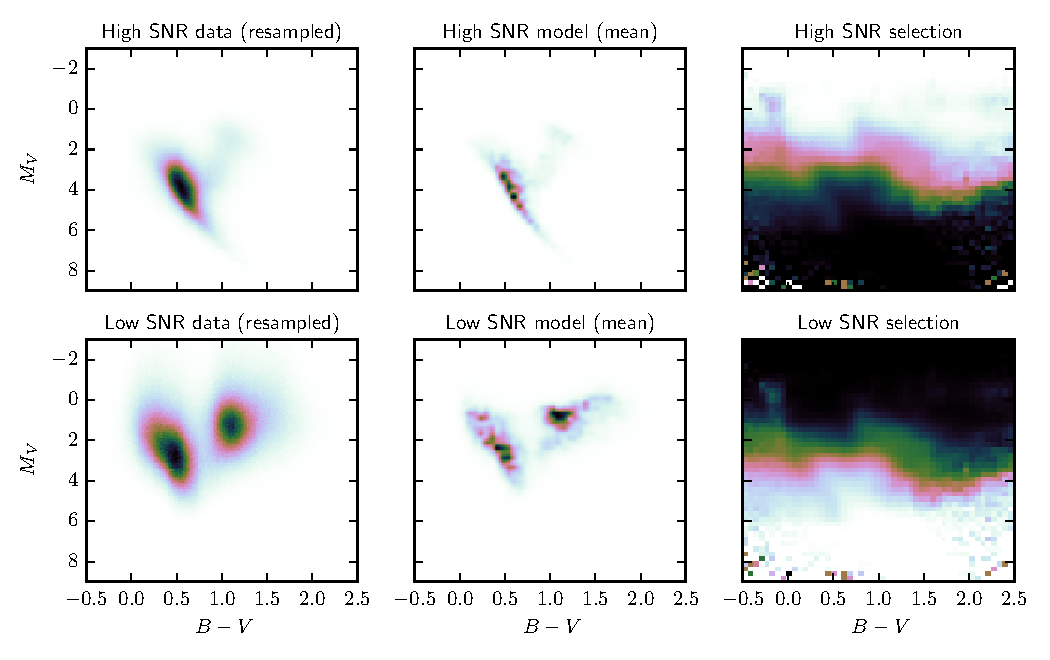
\includegraphics[width=15.9cm]{colmagdiag_othersamples.pdf}
\caption{Same as \figref{fig:colmagdiag_mainsample} for with the main sample split based on parallax SNR. This highlights the contributions of the stars with the `best' and `worst' parallaxes to the color--magnitude diagram, and the importance of using a correct scheme for inferring the latter in the presence of significant observational errors. The right panels show the probability of detecting sources in both subsamples (approximated by resampling the data), which demonstrates how one misses a significant fraction of color--magnitude space by applying parallax SNR cuts. It is by using all of the objects, not only high-SNR ones, that a satisfactory color--magnitude diagram can be inferred.}
\label{fig:colmagdiag_othersamples}
\end{figure}

\begin{figure}
\hspace*{-3mm}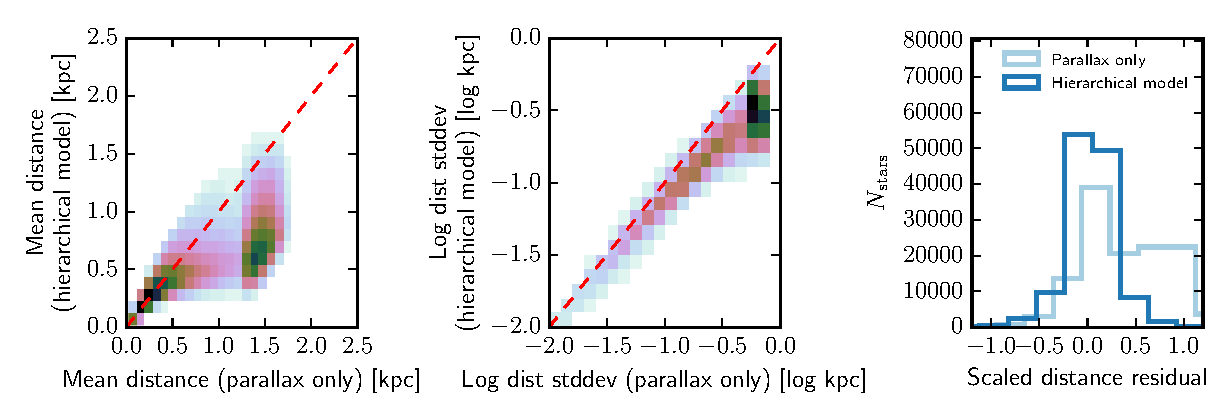
\includegraphics[width=15.8cm]{cv_metrics.pdf}
\caption{Mean, standard deviation, and scaled residuals (truth - mean estimate, divided by standard deviation) of the distances in our validation sample, based on the posterior distributions.
Given the more significant levels of noise the distance are more significantly improved than in our main sample. 
The mean residuals are not zero due to the non-Gaussianity of the posterior distributions.}
\label{fig:cv_metrics}
\end{figure}

\begin{figure}
\hspace*{-3mm}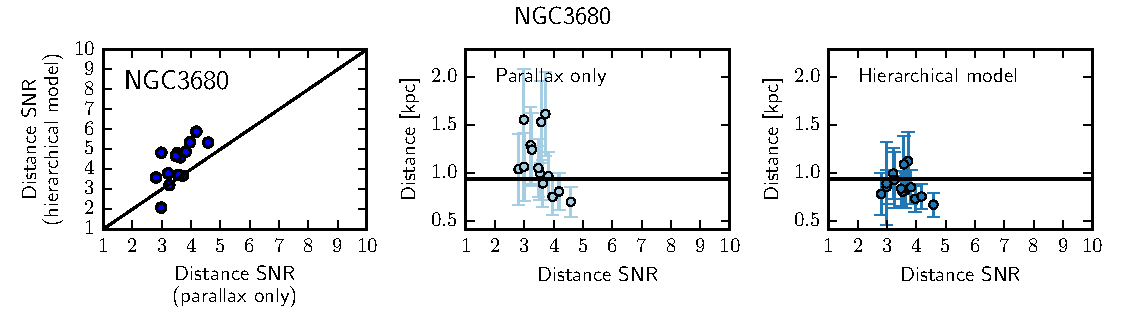
\includegraphics[width=15.8cm, trim = 0cm 1.65cm 0cm 0.65cm, clip]{NGC3680_metrics}
\hspace*{-3mm}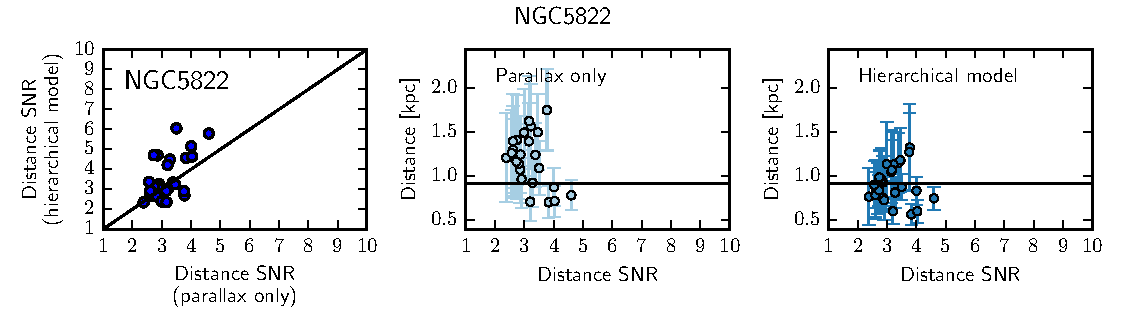
\includegraphics[width=15.8cm, trim = 0cm 1.65cm 0cm 0.65cm, clip]{NGC5822_metrics}
\hspace*{-3mm}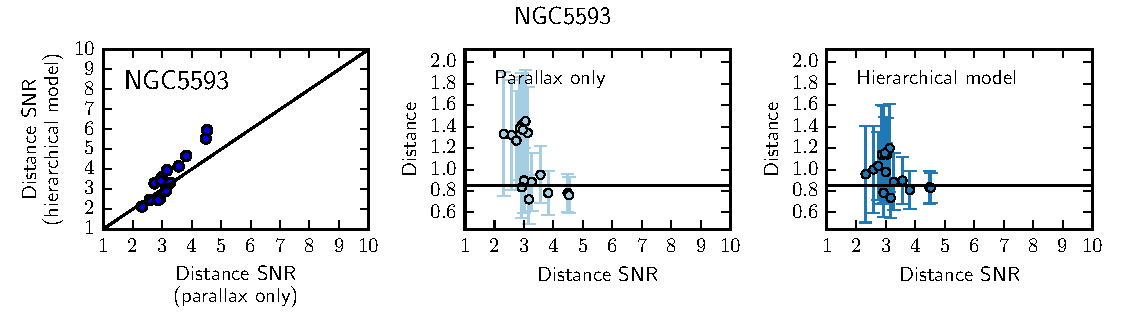
\includegraphics[width=15.8cm, trim = 0cm 1.65cm 0cm 0.65cm, clip]{NGC5593_metrics}
\hspace*{-3mm}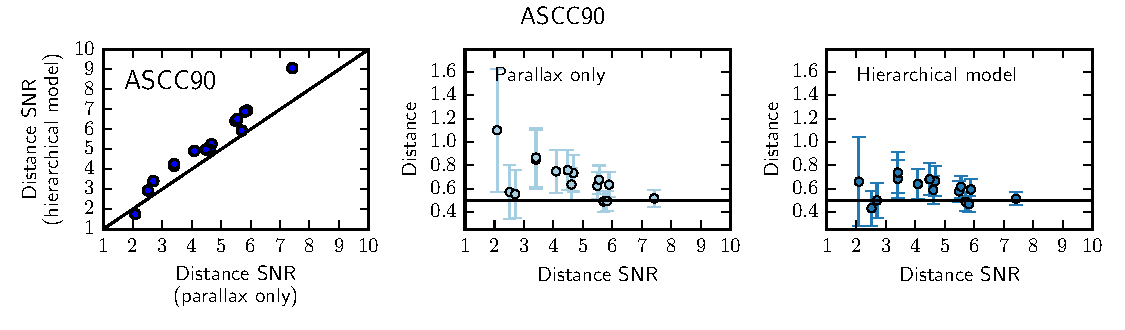
\includegraphics[width=15.8cm, trim = 0cm 1.65cm 0cm 0.65cm, clip]{ASCC90_metrics}
\hspace*{-3mm}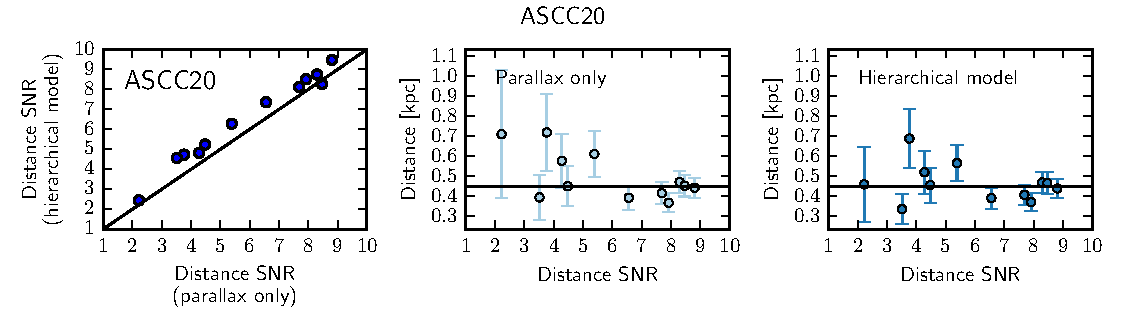
\includegraphics[width=15.8cm, trim = 0cm 1.65cm 0cm 0.65cm, clip]{ASCC20_metrics}
\hspace*{-3mm}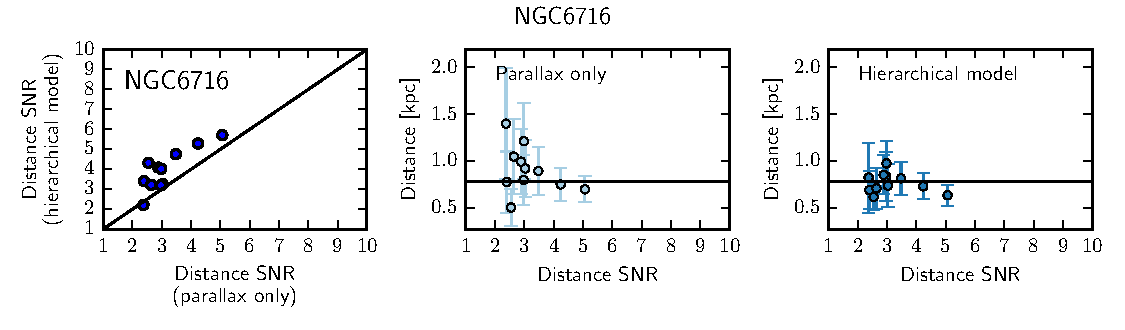
\includegraphics[width=15.8cm, trim = 0cm 0cm 0cm 0.65cm, clip]{NGC6716_metrics}
\caption{Distances estimates of the members of a few open clusters in our data set. The members firmly identified based on position, proper motion and parallax point estimates. }
\label{fig:oc_metrics}
\end{figure}


%%%%%%%%%%%%%%%%%%%%%%%%%%%%%%%%%%%%%%
\section{Conclusion}\label{sec:concl}

Stellar distances are ubiquitous in astronomy and are most directly estimated with parallaxes. 
However, parallax measurements are unreliable for the faintest, most distant objects, which inhabit most of the Galaxy. 
%In particular, the vast majority of the objects detected by Gaia have large parallax uncertainties, which drastically impedes distance estimation. 
We presented a framework for obtaining improved distance estimates with both parallax and color--magnitude information without external data or priors such as stellar models. 
This exploits a well-known property of probabilistic hierarchical models: by utilizing the wealth of information concealed in millions of data points (the noisy and less noisy ones), one can model the underlying distributions and in turn improve the quality of the individual parameter estimates. 
We presented a version of this idea where the color--magnitude distribution of stars is directly inferred from noisy parallax and magnitude measurements via an efficient parameter inference scheme.
We applied this methodology to Gaia data and demonstrated that it leads to significant improvements in the distance estimates, specifically for the faintest, most distant objects.

The framework described here includes a number of simplifying assumptions. 
First, we used uniform distance priors and described the color--magnitude diagram as a mixture of Gaussian kernels with fixed positions and widths.
Those two assumptions could easily be relaxed without affecting our inference methodology.
Second, we ignored selection effects that may distort the color--magnitude diagram and the distance distribution.
Those could be incorporated but require external data and modifications to the sampling method.
Third, we neglected the dependency of the color--magnitude on other properties (\eg galactic latitude), and we performed the magnitude reddenning corrections using existing three-dimensional dust maps evaluated at the parallax-based distance point estimates.
Our framework could also support those extensions with minor technical improvements.
However, in order to fully take advantage of the available data, one should jointly \textit{infer} the three-dimensional distribution of dust and stellar density, and compare with results based on physical models and priors.
This requires more substantial technical developments due to the large number of interlaced parameters.
We intend to explore this avenue in future work.


%%%%%%%%%%%%%%%%%%%%%%%%%%%%%%%%%%%%%%
\acknowledgments

BL was supported by NASA through the Einstein Postdoctoral Fellowship (award number PF6-170154).
DWH was partially supported by the NSF (AST-1517237) and the Moore--Sloan Data Science Environment at NYU.

This project was developed in part at the 2016 NYC Gaia Sprint, hosted by the Center for Computational Astrophysics at the Simons Foundation in New York City.

This work has made use of data from the European Space Agency (ESA) mission Gaia (\url{http://www.cosmos.esa.int/gaia}), processed by the Gaia Data Processing and Analysis Consortium (DPAC, \url{http://www.cosmos.esa.int/web/gaia/dpac/consortium}). Funding for the DPAC has been provided by national institutions, in particular the institutions participating in the Gaia Multilateral Agreement.

This research was made possible through the use of the AAVSO Photometric All-Sky Survey (APASS), funded by the Robert Martin Ayers Sciences Fund.



%%%%%%%%%%%%%%%%%%%%%%%%%%%%%%%%%%%%%%


\bibliography{bib}

%% %%%%%%%%%%%%%%%%%%%%%%%%%%%%%%%%%%%%
\end{document}
%% %%%%%%%%%%%%%%%%%%%%%%%%%%%%%%%%%%%%
